\documentclass[tikz,border=12pt]{standalone}
\usepackage[T1]{fontenc}
\usepackage{mathpazo}
\usepackage{amsmath,amssymb}
\usetikzlibrary{arrows.meta, positioning, calc}

\definecolor{stblue}{HTML}{7B97AD}
\definecolor{rwgold}{HTML}{B8995E}
\definecolor{sage}{HTML}{7A9A7E}
\definecolor{dkbrown}{HTML}{3D3530}
\definecolor{wmgray}{HTML}{7B7067}
\definecolor{cream}{HTML}{F9F6F0}
\definecolor{border}{HTML}{D4C9B8}
\definecolor{terracotta}{HTML}{C47A6A}
\definecolor{lavender}{HTML}{907EA0}

\begin{document}
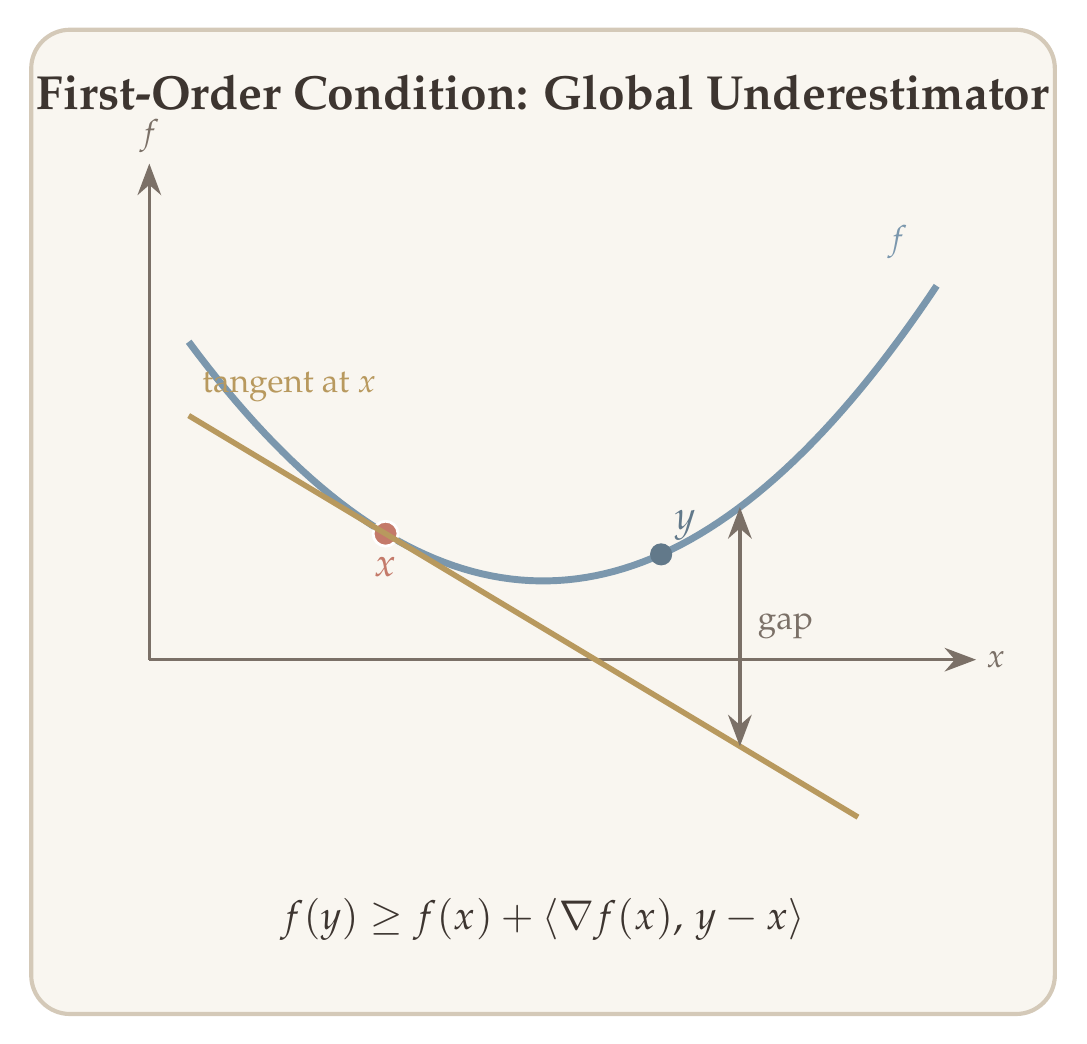
\begin{tikzpicture}[>={Stealth[length=4mm, width=3mm]}]

% Background — expanded vertically to fit equation below the plot
\fill[cream, rounded corners=14pt] (-0.5,-3.0) rectangle (12.5,9.5);
\draw[border, line width=1.5pt, rounded corners=14pt] (-0.5,-3.0) rectangle (12.5,9.5);

% Title
\node[text=dkbrown, font=\LARGE\bfseries] at (6,8.7) {First-Order Condition: Global Underestimator};

% Axes — raised slightly so tangent line stays above equation area
\draw[wmgray, line width=1pt, ->] (1.0,1.5) -- (11.5,1.5) node[right, font=\large, text=wmgray] {$x$};
\draw[wmgray, line width=1pt, ->] (1.0,1.5) -- (1.0,7.8) node[above, font=\large, text=wmgray] {$f$};

% Convex curve: f(x) = 0.15*(x-6)^2 + 2.5
\draw[stblue, line width=2.5pt, domain=1.5:11.0, samples=80]
  plot (\x, {0.15*(\x-6)*(\x-6) + 2.5});
\node[text=stblue, font=\large] at (10.5,6.8) {$f$};

% Tangent point at x0=4: f(4) = 0.15*4+2.5 = 3.1, f'(4) = 0.3*(4-6) = -0.6
\coordinate (x0) at (4, 3.1);
\fill[terracotta] (x0) circle (4.5pt);
\draw[white, line width=1pt] (x0) circle (4.5pt);
\node[text=terracotta, font=\Large\bfseries, below=5pt] at (x0) {$x$};

% Tangent line: y = 3.1 + (-0.6)*(t-4) = 5.5 - 0.6t
% At t=1.5: y = 5.5-0.9 = 4.6;  At t=10: y = 5.5-6.0 = -0.5
% Clip to keep above y=1.5 (axis level): t where y=1.5: 5.5-0.6t=1.5 => t=6.67
\draw[rwgold, line width=2pt] (1.5,{5.5-0.6*1.5}) -- (10.0,{5.5-0.6*10.0});

% Point y on the curve at x=7.5: f(7.5) = 0.15*2.25+2.5 = 2.8375
\coordinate (ypoint) at (7.5, {0.15*(7.5-6)*(7.5-6)+2.5});
\fill[stblue!80!black] (ypoint) circle (4pt);
\node[text=stblue!80!black, font=\Large\bfseries, above right=2pt] at (ypoint) {$y$};

% Gap arrow at x=8.5: curve y = 0.15*(8.5-6)^2 + 2.5 = 0.9375+2.5 = 3.4375
% tangent: 5.5-0.6*8.5 = 0.4 — below axis, so use x=7 instead
% At x=7: curve = 0.15*1+2.5 = 2.65; tangent = 5.5-4.2 = 1.3
% Use x=8: curve = 0.15*4+2.5 = 3.1; tangent = 5.5-4.8 = 0.7 — below axis
% Use x=7: 2.65 vs 1.3
\draw[wmgray, line width=1.2pt, <->] (8.5, {0.15*(8.5-6)*(8.5-6)+2.5}) -- (8.5, {5.5-0.6*8.5});
\node[text=wmgray, font=\large, right=3pt] at (8.5, {0.5*(0.15*(8.5-6)*(8.5-6)+2.5 + 5.5-0.6*8.5)}) {gap};

% Key inequality label — well below the axes
\node[text=dkbrown, font=\Large, align=center] at (6,-1.8)
  {$f(y) \geq f(x) + \langle \nabla f(x),\, y - x \rangle$};

% Tangent line label
\node[text=rwgold, font=\large, above right=2pt] at (1.5,{5.5-0.6*1.5})
  {tangent at $x$};

\end{tikzpicture}
\end{document}
